\section{Projektablauf}

\subsection{Anforderungsdefinitionen}

\subsubsection{Ausgangssituation und Zielsetzung}
\label{subsubsec:ziel}
Das Ziel ist es, eine Applikation zu entwickeln, die es Einrichtungen der Behinderten- und Altenhilfe ermöglicht,
die langfristige Betreuungsplanung mit der Tagesdokumentation zu verknüpfen. Es sollen Ereignisse aus dem Tagesgeschehen,
die in der Tagesdokumentation der Wohngruppe / des Pflegeheims erfasst werden,
der Betreuungsplanung des betroffenen Bewohners zugeordnet werden können.
Damit soll doppelter Dokumentationsaufwand verhindert werden.
Die Software soll in stationären und ambulanten Einrichtungen der Behindertenhilfe in Baden Württemberg eingesetzt werden. 
Diese Einschränkung ergibt sich aus der Implementierung der Betreuungsplanung. Diese Version orientiert sich an dem aktuell in Baden Württemberg
geltenden 
Standard, dem Metzler-Verfahren. 
Die Software soll vorwiegend von pädagogischen Fachkräften benutzt werden. Entsprechend den individuellen Arbeitsabläufen in den 
Einrichtungen der Behindertenhilfe ist auch eine Bedienung durch Personal auf Leitungsebene (Heimleitung) denkbar\cite{Pflichtenheft}.

Die fachlichen Anforderungen an die \EBP wurden gemeinsam mit Herrn Martin Zimmer (Koordinator Unternehmensbereich II des DRK-Sozialwerks in
Bernkastel-Wittlich) erarbeitet und ausformuliert. Ergebnis dieser Arbeit sind die folgenden User Stories.

\subsubsection{User Stories}
\label{subsubsec:userstories}
User Stories sind ein Ansatz aus der Agilen Softwareentwicklung, um die Anforderungen verschiedener User an die Software zu definieren. Die
Formulierung einer User Story erfolgt nach folgendem Template \cite{Wikipedia_User_Story}:
\begin{lstlisting}
As a <role>, I want <goal/desire> so that <benefit>
\end{lstlisting}
Oder in der verkürzten Form:
\begin{lstlisting}
As a <role>, I want <goal/desire>
\end{lstlisting}
User Stories, die thematisch im Zusammenhang stehen werden unter einem Epic zusammengefasst. Die Sprache sollte bei der Formulierung
 von Epic und User Stories aus der Lebenswelt des Kunden stammen. Die Anforderungen an die \EBP wurden in folgende Epic und User Stories aufgeteilt:
\newline

\begin{longtable}{| p{0.25\textwidth}|p{0.05\textwidth}|p{0.7\textwidth} | }
  \hline
 \textbf{Epic} & \textbf{Nr.} & \textbf{User Story} \\
  \hline
\multirow{4}{0.25\textwidth}{Die persönlichen Daten eines Klienten sollen digital verwaltet werden} & 1 & Als Pflegekraft kann ich die Kontaktdaten eines Klienten anzeigen lassen und auch bearbeiten.  \\
  \cline{2 -3}
& 2 & Als Pflegekraft kann ich Informationen über die Leistungsträger der Klienten in meinem Verantwortungsbereich anzeigen lassen und
auch bearbeiten.\\
   \cline{2 - 3}
& 3 & Als Pflegekraft kann ich für die Klienten in meinem Verantwortungsbereich anzeigen lassen, welche freiheitseinschränkenden
Maßnahmen richterlich angeordnet werden, um Rechtssicherheit bei meiner Arbeit zu erlangen.\\
   \cline{2 - 3}
& 4 & Als Pflegekraft kann ich die gesetzliche Betreuung und die institutionelle Bezugsbetreuung anzeigen lassen und auch bearbeiten.\\
  \hline
\multirow{3}{0.25\textwidth}{Für jeden Klienten können mehrere Projekte organisiert werden, die eine pädagogische Zielsetzung haben} & 5 & Als für ein Projekte verantwortlicher Mitarbeiter kann ich neue Projekte anlegen \\
 \cline{2 - 3}
  & 6 & Als für ein Projekte verantwortlicher Mitarbeiter kann ich pädagogische Ziele für ein Projekt definieren \\
   \cline{2 - 3}
  & 7 & Als Pflegekraft kann ich Textfragmente aus der Zielsetzung oder der Projektbeschreibung in einen bestimmten
Bereich der Betreuungsdokumentation übertragen, um den Fortschritt und die Zielerreichung der Langzeitplanung einfach dokumentieren zu können.\\
 \hline
\multirow{4}{0.25\textwidth}{Bei Besprechungen mit einem Klienten müssen Protokolle erstellt werden. Diese Protokolle sollen Teil der \EBP sein.} & 8 & Es können für jeden Klienten mehrere Protokolle angelegt werden. \\
\cline{2 - 3}
 & 9  & Bei jedem Protokoll sind die Teilnehmer und das Protokolldatum ersichtlich. \\
\cline{2 - 3}
& 10 & Ein oder mehrere Teilnehmer können als Protokollant markiert werden \\
\cline{2 - 3}
& 11 & Als Pflegekraft kann ich Textfragmente aus dem Protokolltext in einen bestimmten
Bereich der Betreuungsdokumentation übertragen, um den Fortschritt und die Zielerreichung der Langzeitplanung einfach dokumentieren zu können.\\
\hline
\multirow{4}{0.25\textwidth}{Für jeden Klienten solle es eine Betreuungsdokumentation für verschiedene Lebensbereiche geben.}& 12 & Als Bezugsbetreuer kann ich in jedem Lebensbereich den Hilfebedarf eines Klienten kategorisieren.\\
\cline{2 - 3}
& 13 & Als Bezugsbetreuer kann ich in jedem Lebensbereich den Hilfebedarf eines Klienten prosaisch näher beschreiben.\\
\cline{2 - 3}
& 14 & Als Bezugsbetreuer kann ich in jedem Lebensbereich pädagogische Ziele definieren, um eine zielgerichtete pädagogische Arbeit zu
ermöglichen.\\
\cline{2 - 3}
& 15 & Als Pflegekraft kann ich Textfragmente aus anderen Teilen der \EBP an die prosaische Beschreibung der einzelnen Lebensbereiche
senden, um den Fortschritt und die Zielerreichung der Langzeitplanung einfach dokumentieren zu können.\\
\hline
\multirow{2}{0.25\textwidth}{Es gibt ein Gruppenbuch, in dem die tagesaktuellen Geschehnisse einer Wohngruppe dokumentiert werden.}& 16 & Als Pflegekraft kann ich ein Ereignis auf einer Wohngruppe in meinem Verantwortungsbereich mit de \EBP dokumentieren, um eine
lückenlose Kommunikation mit meinen Kollegen zu gewährleisten.\\
\cline{2 - 3}
& 17 & Als Pflegekraft kann ich Textfragmente aus einem Ereignis in einen bestimmten
  Bereich der Betreuungsdokumentation übertragen, um den Fortschritt und die Zielerreichung der Langzeitplanung einfach dokumentieren zu können.\\
 \hline
 Die Abwesenheit eines Klienten von der Wohngruppe über einen Zeitraum größer gleich einem Tag muss zur Abrechnung mit dem Leistungsträger
dokumentiert werden. & 18 & Als Pflegekraft kann ich die Abwesenheit eines Klienten mit der \EBP dokumentieren, um eine der Verwaltung eine einfache
Abrechnung zu ermöglichen.\\
 \hline
\end{longtable}

\subsubsection{Qualitätssicherung zur Einhaltung der Anforderungsdefinitionen}
Um die Benutzbarkeit sicherzustellen wurden eine Reihe von Usability-Tests durchgeführt. KRUG beschreibt den Stellenwert von Usability-Tests sehr treffend: \\
''Wenn Sie an einer Seite auch nur einige Wochen gearbeitet haben, können Sie sie nicht mehr unbedarft betrachten. Sie wissen zu viel. Der einzige Weg, um herauszufinden, ob sie wirklich funktioniert, sind Tests\cite[S. 133]{Usability}.'' \\
\noindent
Dies gilt natürlich nicht nur für Websites sondern auch für das Erstellen jeder anderen grafischen Oberfläche. Angelehnt an den Scrum artigen Entwicklungsprozess war auch der Usability-Test Prozess mehrstufig.

\paragraph*{Ablauf:}
\begin{description}

        \item[Phase 1] Nach der grundlegenden Gestaltung der grafischen Oberfläche ohne funktionale Logik wurden \textit{Tests zum Kapieren} mit verschiedenen Testpersonen durchgeführt. Diese \textit{Tests zum Kapieren} sollen feststellen, ob der Nutzer die Bedienkonzepte, wie z.B. die Navigation, und Absichten der Anwendung versteht\cite[Vgl. S. 144]{Usability}.

        \item[Phase 2] In dieser Phase des Testprozesses waren die getesteten Masken vollständig implementiert und wurden an Hand von \textit{Schlüsselaufgaben} getestet. ''Tests mit Schlüsselaufgaben bedeuten, dass Sie den Usern eine Aufgabe stellen und dann beobachten, wie gut sie zurechtkommen\cite[Vgl. S. 144]{Usability}.'' Die \textit{Schlüsselaufgaben} wurden so definiert, dass mit ihrer Überprüfung gleichzeitig die Umsetzung der User Stories überprüft wurde. Damit erfolgte durch die Usability-Tests auch eine Überprüfung des Erfüllungsgrads der Anforderungsdefinitionen. Folgende Schlüssel-aufgaben wurden für die entsprechenden User Stories (Siehe Nummer) definiert:

        \begin{enumerate}
		\item Finde das Geburtsdatum von Waldemar Fried heraus. 
		\item Füge die Deutsche Rentenversicherung als Leistungsträger bei Melinda Müller hinzu.
		\item Prüfe, wann Melinas Verfügung für die Fixierung abläuft.
		\item Finde heraus, wie die gesetzliche Betreuerin von Hans Müller heißt und wo Sie wohnt.
		\item Lege ein neues Projekt für Hans Müller an, 
		\item das die Förderung seiner Selbstständigkeit zum Ziel hat.
		\item Übertrage diese Ziele in ein entsprechendes Feld der Betreuungsplanung von Willfred Schuster.
		\item Lege ein Protokoll für ein Gespräch mit Herman Hinz über sein Verhalten am Mittagstisch an.
		\item Füge Marlene Friedrich und Klaus Müller als Teilnehmer hinzu.
		\item Markiere Marlene Friedrich als Protokollantin.
		\item Übertrage das Ergebnis des Gesprächs mit Melinda vom 19 März 2012 in ihre Betreuungsplanung, Kategorie "Partnerschaften"
		\item Stufe den Hilfebedarf von Maria Schreiber im Lebensbereich "Einkaufen" neu ein,
		\item und beschreibe den Hilfebedarf genauer.
		\item Definiere ein pädagogisches Ziel, um diesen Hilfebedarf zu ändern.
		\item Übertrage die Beschreibung aus dem Projekt "Einkaufen gehen lernen" von Maria Schreiber in die Betreuungsplanung.
		\item Finde heraus, was am 23.12.2011 auf der Wohngruppe vorgefallen ist.
		\item Übertrage den Sturz von Waldemar Fried in die Betreuungsplanung.
		\item Melde Waldemar Fried für den heutigen Tag Abwesend, da er im Urlaub bei seinen Eltern ist.
        \end{enumerate}

\end{description}

\paragraph*{Ergebnisse:}
\begin{description}

\item[Phase 1:]

\item[Phase 2:] In dieser Phase wurde die Stellen offen gelegt, an denen den Usern das Bedinkonzept nicht deutlich wurde.
Als Ergebnis wurde zum Beispiel beim \textit{TextTransfer} ein Hilfebutton eingefügt, der eine kleines PopUp mit kurzer Hilfestellung anzeigt.
Häufige Problemstellungen waren auch falsche oder uneinheitliche Benennungen von Menüpunkten und Inhalt. Diese Fehler waren sehr dankbar, da leicht zu beheben und verdeutlichen noch einmal den Stellenwert von Usability Tests. Das Konzept, dass \EBP immer einen aktiven Bewohner und eine aktive Wohngruppe hat, war die größte Hürde für die User.
Die Informationen über die aktuell aktive Wohngruppe und den aktiven Bewohner werden in einem Informationswidget im oberen Bereich der Anwendung visualisiert (siehe dazu Kapitel \ref{sec:beschreibung}). Dort können die aktiven Elemente auch geändert werden. Bei jedem Test wurde das Bedienkonzept erst klar, als der User das Infowidget endeckte und seine Funktionen  ausprobierte. In allen Fällen war das 
Konzept nach kurzem Experimentieren klar. Eine Verbesserung der Bedienbarkeit sollte jedoch an diesem Widget ansetzten. Die vollständigen Ergebnisse finden sich im Anhang in Form von Protokollen oder in Form von Screencasts mit Tonaufnahmen der Testsitzungen.

\end{description}


\subsection{Scrum}
Um die Komplexität des Projekts zu reduzieren wurde ein iteratives Vorgehensmodell gewählt, dass sich stark an dem \textit{Scrum Framework}
orientierte. Organisatorische Elemente des \textit{Scrum Frameworks}, wie das \textbf{Sprint Planning}, das \textbf{Sprint Review} und die
\textbf{Sprint Retrospective} wurden nicht umgesetzt. Der Fokus bei unserer Adaption des \textit{Scrum Frameworks} lag in der Anforderung, aus einer
globalen Zielsetzung möglichst strukturierte Arbeitspakete zu generieren. Der klassische Scrumzyklus, visualisiert in Abbildung \ref{ScrumFramework},
eignet sich für diese Anforderung durch seine Methodik, vor allem die Definition in User Stories und die Gliederung dieser in einem
\textbf{Backlog}, in besonderer Weise.\\

\begin{figure*}[htp]
	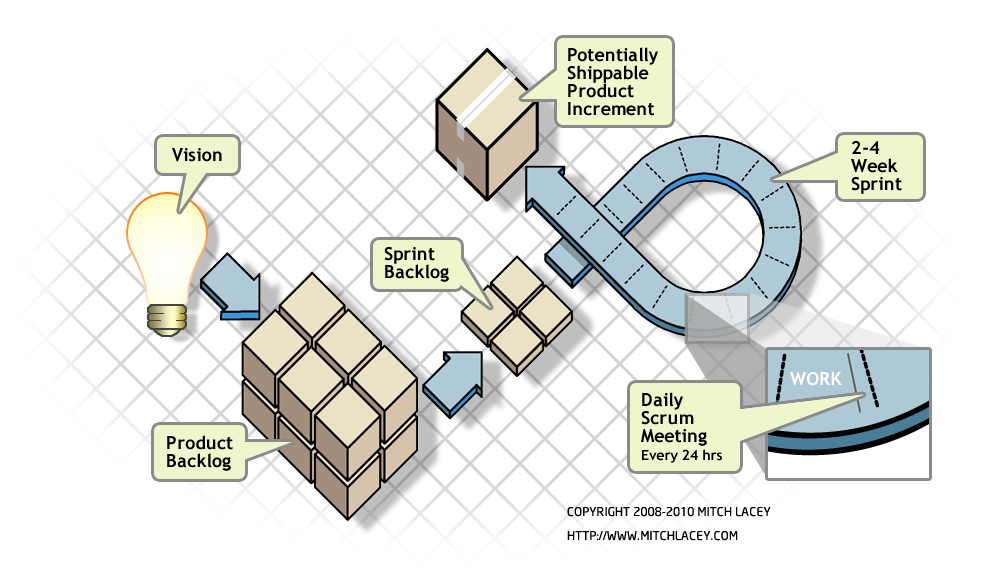
\includegraphics[width=\textwidth]{ScrumFrameworkFlow}
	\caption{Scrum Framework}
	\label{ScrumFramework}
\end{figure*}

Unsere \textbf{Vision} war die in Kapitel \ref{subsubsec:ziel} beschriebene Zielsetzung. Der Dokumentationsaufwand in der Behinderten- und Altenhilfe
soll durch die \EBP verringert werden. Das \textbf{Product Backlog} bildeten die gesamten User Stories, die bei ihrer Erstellung priorisiert wurden.
Das \textbf{Sprint Backlog} bestand in jeder Iteration aus drei bis vier User Stories. Dieses \textbf{Sprint Backlog} wurde in innerhalb einer
\textbf{Sprint} Phase abgearbeitet. Als Zeitraum für einen \textbf{Sprint} waren vier Wochen geplant, so dass nach fünf \textbf{Sprint} Phasen das
Projekt fertig entwickelt sein sollte und vier Wochen als Puffer verbleiben sollten. Zur Visualisierung des \textbf{Product} und \textbf{Sprint
Backlogs} wurden die Werkzeuge der Plattform \url{github.com} genutzt. Die Plattform bietet neben der Versionskontrolle durch das verteilte
Versionsverwaltungswerkzeugs \textit{git} auch die Möglichkeit Meilensteine mit zugehörigen Aufgaben zu definieren und diese einzelnen
Projektteilnehmern zuzuordnen. Das \textbf{Daily Scrum Meeting} wurde nicht in der vom \textit{Scrum Frameworks} vorgesehen Regelmäßigkeit und
Verbindlichkeit durchgeführt. In der ex post Betrachtung stellt sich dies als Fehler heraus. Schwierigkeiten bei der Implementierungen hätten sich
bei regelmäßiger Rücksprache untereinander sicher schneller lösen lassen. Auch eine stärkere Verbindlichkeit gegenüber den Projektzielen hätte sich
durch kontinuierliche Reflexion erzeugen lassen und zu einem besseren Produkt geführt. Eine \textbf{Shippable Product Increment} war nicht das Ziel
einer \textbf{Sprint} Phase. Allerdings sollten die User Stories des jeweiligen \textbf{Sprint Backlogs} am Ende einer \textbf{Sprint} Phase
vollständig umgesetzt sein, inklusive durchlaufener Qualitätssicherung.  
